\documentclass[a4paper,11pt]{article}
\pdfoutput=1 % if your are submitting a pdflatex (i.e. if you have
             % images in pdf, png or jpg format)

\usepackage{jcappub} % for details on the use of the package, please
                     % see the JCAP-author-manual

\usepackage[T1]{fontenc} % if needed



\title{\boldmath Physics-Guided Inversion Networks for QUBIC Map-Making }


%% %simple case: 2 authors, same institution
%% \author{A. Uthor}
%% \author{and A. Nother Author}
%% \affiliation{Institution,\\Address, Country}

% more complex case: 4 authors, 3 institutions, 2 footnotes
\author[a]{L. Kardum,}
\author[a]{T. Laclavère,}
\author[a]{J-Ch. Hamilton,}
\author[a]{A. Huchet,}
\author[a]{and S. Torchinsky}

% The "\note" macro will give a warning: "Ignoring empty anchor..."
% you can safely ignore it.

\affiliation[a]{Universite de Paris, CNRS, Astroparticule et Cosmologie, \\ F-75006 Paris, France}

\abstract{Reconstructing sky maps from time-ordered data is an ill-conditioned inverse problem for the QUBIC bolometric interferometer, usually solved through  forward modeling which can be computationally expensive due to its iterative nature. Here we present an alternative approach that factorizes the QUBIC measurement operator into individual physical processes and constructs an explicit analytical or pseudo inverse for each. Machine Learning is used to correct only the residual of operators that are fundamentally ill-conditioned, like the interferometric projection. By restricting learned components to the residual of a physically motivated approximate inverse, the resulting model achieves reconstruction comparable to Preconditioned Conjugate Gradient solutions while using orders of magnitude less parameters. We demonstrate the method initially on monochromatic simulated CMB maps and extend it to multi-band spectral-imaging reconstruction, and show how the same differentiable architecture additionally enables estimation of instrumental parameters and propagation of their uncertainties through the inverse chain.}



\begin{document}
\maketitle
\flushbottom

\section{Introduction}
\label{sec:intro}

The detection of B-modes and constraint of the tensor-to-scalar ratio $r$ from measurements of the Cosmic Microwave Background (CMB) would confirm the existence of primordial gravitational waves. However, recovering the CMB from the data of a ground-based experiment is an inverse problem, complicated by atmosphere, foregrounds, and the instrumental effects.

The QUBIC experiment (Q \& U Bolometric Interferometer for Cosmology) is a bolometric interferometer, combining the advantages of both technologies to detect the B-mode polarization of the CMB \cite{hamilton2022qubic1, mousset2022qubic2}. As described in Section~\ref{sec:instrument}, the measurement process is a sequence of instrumental operations, including modulation by a rotating half-wave plate and interferometric projection of the scanned sky. Most of the operators describing this process are individually well understood, but several are ill-conditioned or non-invertible, which makes solving the full inverse problem numerically challenging.

Conventional data-driven machine learning models can offer fast and precise solutions for similar problems, but they usually lack interpretability. Moreover, they cannot easily be generalized to related problems or other experiments. In this work we propose a physics-guided method: instead of learning the full TOD-to-sky inverse end-to-end, we factorize the QUBIC acquisition operator into its constituent physical processes (Section~\ref{sec:modular}), construct an approximate inverse, and restrict machine learning to optimize only on parameters we understand well with a limited predefined architecture. This uses the learning capacity of neural networks only where necessary.

We first validate this approach on monochromatic reconstruction (Section~\ref{sec:validation-mono}), where it is compared with the standard Preconditioned Conjugate Gradient pipeline. Because every stage of the resulting network corresponds to a named physical operator and not an unknown function, the same differentiable pipeline is used to estimate instrumental constants as uncertain quantities, shown in Section~\ref{sec:probabilistic}). This is not possible with either the conventional PCG pipeline or end-to-end reconstruction neural networks.


\section{The QUBIC Instrument}
\label{sec:instrument}

The Q \& U Bolometric Interferometer for Cosmology (QUBIC) is a ground-based instrument located at Alto Chorrillos near Salta, Argentina, at an altitude of 4900 meters above sea level \cite{hamilton2022qubic1}. This high altitude site was
chosen for its dry and stable atmospheric conditions, which minimize the emission and fluctuations of atmospheric water vapor at millimeter wavelengths \cite{hamilton2022qubic1}. 

\par
QUBIC is a bolometric interferometer, combining reliability of bolometers with spectral imaging capability of interferometry, previously never combined in one CMB experiment \cite{hamilton2022qubic1, mousset2022qubic2}. Bolometry with large arrays of transition-edge sensor (TES) detectors enables high sensitivity. Interferometry allows it to synthesize a frequency-dependent beam pattern whose spatial properties encode spectral information, enabling spectral-imaging. The instrument currently operates in a technological demonstrator configuration (TD) and is being upgraded to the full instrument (FI), which will use a wide frequency band (UWB) and 992 TES bolometers \cite{torchinsky2022qubic3, hamilton2022qubic1}.

\begin{figure}[h]
\centering 
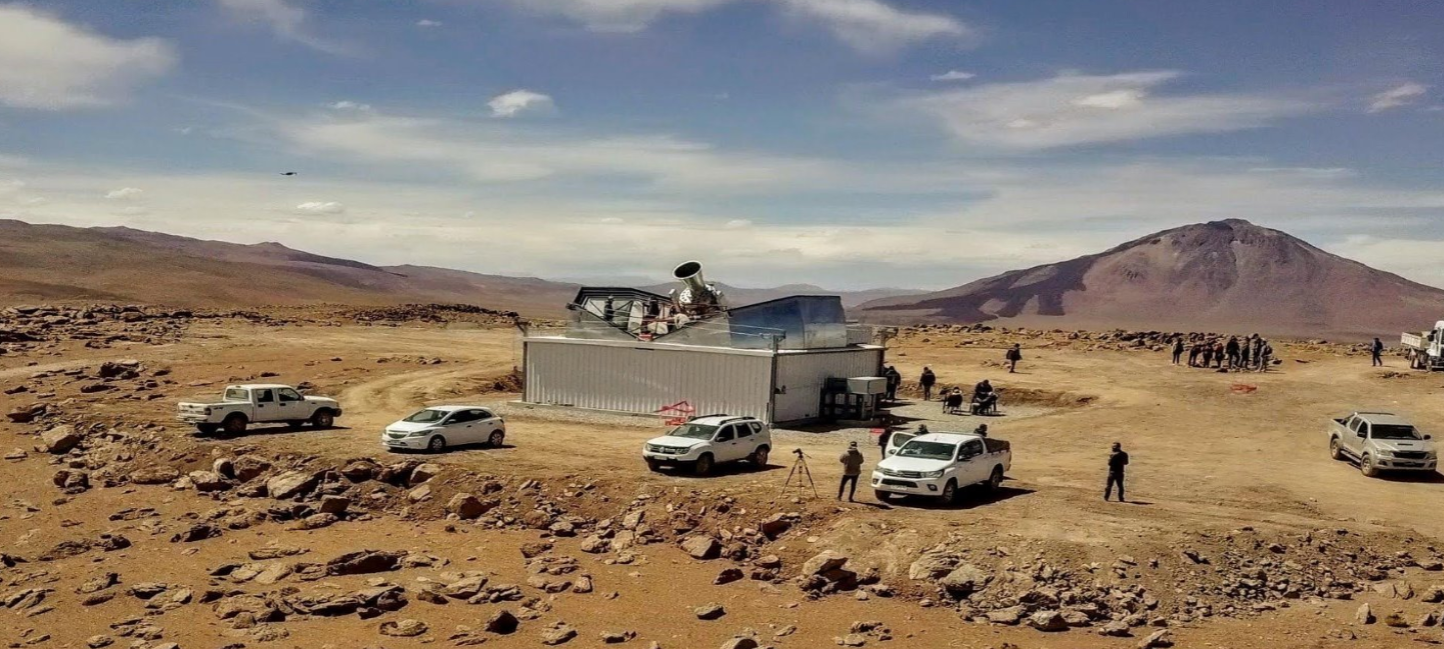
\includegraphics[width=.85\textwidth]{instrument-at-arg.png}
\caption{\label{fig:instrument-at-arg} View of the QUBIC instrument installed at the Alto Chorillos site in Argentina.}
\end{figure}

\subsection{Acquisition in QUBIC}
\label{subsec:acquisition}

The physical process of detection in QUBIC is presented here in steps so they can be clearly connected to operators that will be described in Section~\ref{sec:forward}.

\paragraph{Unit conversion.}
The conversion of sky brightness temperature (in $\mu$K) to detector power (in W) is
performed by the unit conversion operator $U$, which applies the derivative of the Planck spectrum evaluated at the center of the band
\cite{mousset2022qubic2}
\begin{equation}
    U = \frac{10^{-6}}{T^2}\,\frac{2\Omega_{\rm pix}\,h\nu^3}{c^2}
    \frac{\left(\frac{h\nu}{kT}\right)^2
    e^{h\nu/kT}}{\left(e^{h\nu/kT}-1\right)^2},
    \label{eq:unit-conversion}
\end{equation}
where $h$ is Planck's constant, $k$ is Boltzmann's constant, $\nu$ is the frequency, and $\Omega_{\rm pix}$ is the solid angle of a HEALPix pixel. 

\paragraph{Horn aperture and filtering.}
Radiation enters the cryostat through a polyethylene window and passes through a series of low-pass filters to keep only frequencies in the desired band, before reaching the instrument interior which is cooled to cryogenic temperatures of 320~mK to minimise 
thermal noise \cite{torchinsky2022qubic3}. A bandpass filter selects the observing band between around 150~GHz and 220~GHz for the focal plane of the FI \cite{hamilton2022qubic1}. This spectral filtering is described by the operator $F$. The radiation then enters an array of 400 back-to-back horns arranged on a square grid within a circular aperture \cite{mousset2022qubic2}. Each horn collects radiation from
the sky over its primary beam $B_{\rm prim}(\hat{n},\nu)$. Integrating the collected flux over the aperture area gives the operator $A$, which converts spectral power density (W~Hz$^{-1}$) to total power (W) \cite{mousset2022qubic2}. 

\begin{figure}[h]
\centering 
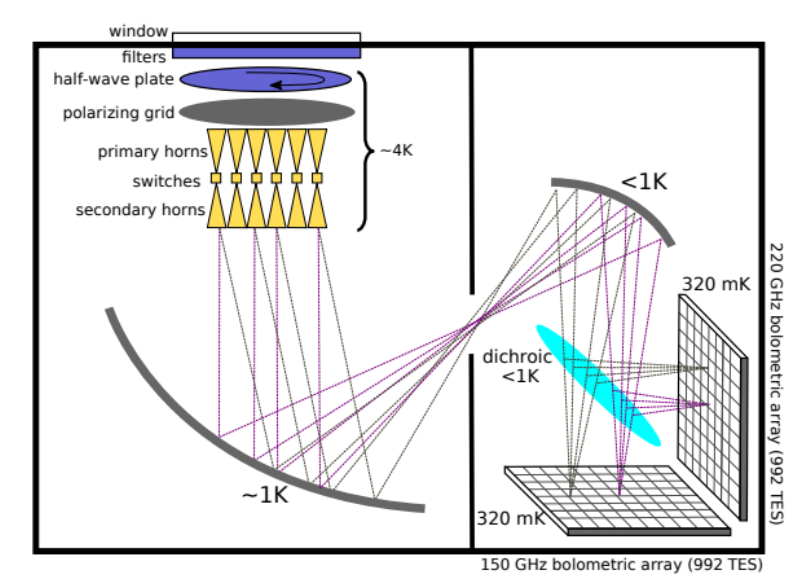
\includegraphics[width=.75\textwidth]{schematic.png}
\caption{\label{fig:schematic} Schematic of the QUBIC optical chain. Radiation enters through the window (top), passes through filters and the half-wave plate, is polarized by the polarizing grid, collected by the horn array, interfered by the mirrors, and detected on the TES focal plane.}
\end{figure}


\paragraph{Half-wave plate and polarizing grid}
Mounted at the entrance of the cryostat is the rotating Half-wave plate 
(HWP) \cite{hamilton2022qubic1}. The HWP is a birefringent element that, when rotated by an angle $\psi(t)$, modulates the incoming Stokes parameters as
\begin{equation}
    H_W(\psi) =
    \begin{pmatrix}
        1 & 0 & 0 \\
        0 & \cos 4\psi(t) & \sin 4\psi(t) \\
        0 & -\sin 4\psi(t) & \cos 4\psi(t)
    \end{pmatrix},
    \label{eq:hwp}
\end{equation}
where the rows correspond to Stokes $I$, $Q$, and $U$ \cite{mousset2022qubic2}. It is continuously rotating at a fixed angular velocity. 

After the HWP, a polarizing filter, described by $P$, transmits radiation of one linear polarization and rejects the orthogonal component. For a polarizer oriented along the instrument axis, the output signal is \begin{equation}
    S = S_I + S_Q \cos 4\psi(t) + S_U \sin 4\psi(t)
    \label{eq:polarizer}
\end{equation}
where the Stokes $(I,Q,U)$ are projected onto a single amplitude per detector and per one time step \cite{mousset2022qubic2}.

\paragraph{Interferometric projection.}
The horn array acts as an interferometer. The radiation from all 400 horns is re-emitted into the back-to-back horn array and combined with a series of mirrors, before
arriving at the focal plane \cite{mousset2022qubic2,
torchinsky2022qubic3}. This produces an interference
pattern on the focal plane, which we call the synthesized beam. In a classical imager, the synthesized beam would be the point-spread function (PSF). Each detector on the focal plane records a sum of signals from multiple directions, weighted by the synthesized beam
pattern. This makes the acquisition process a many-to-one mixing, and is described by the projection operator $L$ in Eq.~\ref{eq:operator-chain}, which maps the pixelized sky
$(N_{\rm pix} \times 3)$ to TOD samples $(N_{\rm det} \times N_{\rm samples} \times 3)$. The structure of $L$ and the properties of the synthesized beam are discussed in detail in
Section~\ref{subsec:spectral-imaging}. 

\paragraph{Flux integration and detector response.}
After the optical combination, the flux density in each detector is integrated over the solid angle of the secondary beam $B_{\rm sec}(r,\nu)$ on the focal plane, described by the operator $D$, and further affected by instrumental transmission
factors coming from optical elements in the cryostat and mirrors, described by the operator $I$ \cite{mousset2022qubic2}.

Finally, the TES bolometers have a finite time response. Each detector does not measure power $x(t)$ instantaneously, but the convolution
\begin{equation}
    y(t) = \int x(t')\,e^{-(t-t')/\tau}\,dt',
    \label{eq:detector-response}
\end{equation}
where $\tau \sim 10$~ms is the detector time constant \cite{mousset2022qubic2}. This convolution is described by the operator $B$.

\subsection{Synthesized Beam and Spectral Imaging}
\label{subsec:spectral-imaging}

The most distinctive property of QUBIC is the multi-peaked synthesized beam produced by the interferometry in the horn array. It enables spectral imaging, but it is also the main challenge in map reconstruction. 

When the 400 horns combine the incoming light, the signal on the focal plane is proportional to the square of the summed electric field from all baselines. For this horn array, this produces a synthesized beam consisting of multiple peaks, whose angular separation is set by the horn spacing and the focal length \cite{mousset2022qubic2}. An arbitrary number of peaks can be considered up to a given diffraction order $k_{max}$. The synthesized beam with nine retained peaks is illustrated in Fig.~\ref{fig:synthesized-beam}. Each detector sample in QUBIC records a
superposition of signals from several directions on the sky at the same time, compared to a single peak PSF measured with conventional imagers. This mixing is the main source of ill-conditioning in the full acquisition operator $H$, as it will be detailed in Sections~\ref{sec:modular} and~\ref{sec:operators}.

\begin{figure}[h]
\centering 
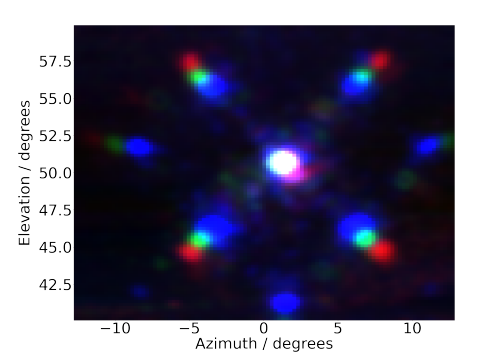
\includegraphics[width=.65\textwidth]{synthesized-beam.png}
\caption{\label{fig:synthesized-beam} The synthesized beam at 130~GHz (red), 150~GHz (green), and 170~GHz (blue). Taken from \cite{torchinsky2022qubic3}.}
\end{figure}

In practice, implementing the full synthesized beam, with thousands of secondary peaks, in the forward operator is computationally expensive and has limited advantages in the map reconstruction. The QUBIC software uses the Gaussian peak approximation, where each peak of the synthesized beam is modeled as a Gaussian with frequency dependence. 

The angular separation between the synthesized beam peaks scales linearly with wavelength, as $\Delta\theta_{\rm peaks} \propto \lambda/d_{\rm
horn}$, where $d_{\rm horn}$ is the horn spacing \cite{mousset2022qubic2}. Separation $\Delta\theta_{\rm peaks}$ at three different wavelengths is seen on Fig.~\ref{fig:synthesized-beam}. This frequency dependence of the synthesized beam encodes spectral information in the TOD because different frequency
components of the sky signal are mixed with different spatial weights, and this mixing can be inverted to recover sky maps at multiple frequencies within a single band. This ability is called spectral imaging \cite{mousset2022qubic2,
regnier2024freqmaps}.

Observation at one frequency is called the monochromatic acquisition, and integrating  over the full band $[\nu_{\rm min}, \nu_{\rm max}]$ gives
\begin{equation}
    d = \int_{\nu_{\rm min}}^{\nu_{\rm max}}
    H_\nu\,s_\nu\,d\nu + n,
    \label{eq:polychromatic}
\end{equation}
where $H_\nu$ is the monochromatic acquisition operator at frequency $\nu$. Spectral imaging approximates the sky as a constant within $N_{\rm rec}$ reconstructed sub-bands
$\{\tilde{s}_{\nu_i}\}_{i=1}^{N_{\rm rec}}$, each centred at frequency $\nu_i$, so that
\begin{equation}
    d \;\approx\; \sum_{i=1}^{N_{\rm rec}} \vec{H}_{\nu_i}\,
    \tilde{s}_{\nu_i},
    \label{eq:spectral-imaging}
\end{equation}
where the sub-band acquisition operator
\begin{equation}
    \vec{H}_{\nu_i} = \sum_{j=1}^{N_{\rm sub}}
    \Delta\nu_{ij}\,H_{\nu_{ij}}\,C_{K_{ij}}
    \label{eq:subband-operator}
\end{equation}
is itself a sum of $N_{\rm sub}$ monochromatic acquisitions within the
sub-band, weighted by $\Delta\nu_{ij}$ and convolved with a Gaussian
kernel $C_{K_{ij}}$ of appropriate resolution \cite{mousset2022qubic2, regnier2024spectral}. Number of sub-bands $N_{\rm sub}$ is chosen large enough to approximate integration, while the choice $N_{\rm rec}$ gives the number of reconstructed maps in both classical map-making and in this approach. The parameter $N_{\rm rec}$ is an important free parameter of spectral imaging, and its maximum is limited by the spectral
resolution of the interferometer, $\Delta\nu/\nu \simeq 1/N_{horns}$, where $N_{horns}$ is the number of horns along one side of the square array \cite{mousset2022qubic2}. 

The forward operator in Eq.~\ref{eq:spectral-imaging} in spectral imaging is a sum of $N_{\rm rec}$ coupled
projection operators, each with a different beam size due to frequency dependence. Recovering $N_{\rm rec}$ sky maps $\{\tilde{s}_{\nu_i}\}$ from a single TOD is an underdetermined problem and is further complicated compared to monochromatic reconstruction only. Using the available information about the synthesized beam at each frequency and careful consideration of interacting pixels allows also the multi-band reconstruction in the inverse modular approach.

The noise of reconstructed sub-band maps is not independent, \cite{regnier2024spectral, mousset2022qubic2}. The structure of the synthesized beam peak mixing introduces correlations between different sub-bands in the noise covariance matrix of the reconstructed maps. These correlations must be accounted for, and we show how to use these constraints in a neural network framework in Section~\ref{sec:architecture-loss}.

\section{Forward Model and Classical Map-Making}
\label{sec:forward}

\subsection{Time-Ordered Data and the Acquisition Operator}
\label{subsec:tod}

In QUBIC, each of the $N_{\rm det}=992$ transition-edge sensors (TES) on the focal planes records time-ordered data (TOD) that results from a
sequence of optical and electronic transformations
applied to the true sky signal $s$. Sky is composed of Stokes maps $s=(I,Q,U)$, pixelized on a HEALPix grid, and $d$ is the
array of all TOD samples for all detectors, so the acquisition is modeled as the linear system
\begin{equation}
    d = Hs + n,
    \label{eq:forward}
\end{equation}
where $H$ is the acquisition operator and $n$ is
instrumental and photon noise.

The acquisition operator $H$ does not correspond to a single physical process but a sequence, and is therefore a composition of operators, each corresponding to one
stage of the mentioned optical and electronic chain between the sky and the
detector readout \cite{mousset2022qubic2}. The acquisition operator can be written as a sequence of operations such as
\begin{equation}
    H \;=\; B \cdot I \cdot D \cdot L \cdot H_W \cdot P \cdot F \cdot A \cdot T \cdot U,
    \label{eq:operator-chain}
\end{equation}
in the order in which they act on the sky (right to left in Eq.~\ref{eq:operator-chain}). The operators in the acquisition process are:
$U$, unit conversion between sky brightness and detector power;
$T$, atmospheric transmission;
$A$, horn aperture integration;
$F$, bandpass filtering;
$P$, the polarizing grid;
$H_W$, the rotating half-wave plate;
$L$, the interferometric projection operator, which maps the
multiply-peaked synthesized beam pattern \cite{mousset2022qubic2}
onto the focal plane and is responsible for the frequency-dependent
spectral-imaging capability of the instrument
\cite{regnier2024freqmaps, regnier2024spectral};
$D$, the flux integration;
$I$, instrumental transmission;
and $B$, the time response of the bolometers. The physical processes of these operators are described in detail in Section~\ref{subsec:acquisition}.

Operators in Eq.~\ref{eq:operator-chain} have different structures: $U$, $T$, $A$, $F$ are diagonal or homothety operators (scalar multiplications);
$P$ and $H_W$ are dense, block-diagonal rotations acting on the three
Stokes maps in each sample; $B$ is a convolution; $D$ and $I$ are diagonal
operators; and $L$ is a sparse, non-square, many-to-one mapping from sky pixels to TOD samples, reflecting how each detector receives light from multiple directions through the synthesized beam \cite{mousset2022qubic2}. 

Filter $F$, aperture $A$, and Unit conversion $U$ are exactly invertible by element-wise division. Because $H_W$ is a rotation matrix in Stokes space, its inverse is simply its transpose, $H_W^{-1} = H_W^T$, and no learning is required for this stage. The polarizer is a projection from three-dimensional Stokes to a scalar and its inverse requires knowledge of the HWP modulation, which is exactly known, making this step analytically invertible. Instrumental transmission $I$ and flux integration $D$ are invertible in the same way as $F$, $A$, and $U$. Bolometer response $B$ is invertible in the Fourier domain and is treated as an approximate-inverse module in our framework (Section~\ref{subsec:detector}). 

Only projection is fundamentally non-invertible while other operators are diagonal or simple convolutions, which motivates the modular inversion strategy that will be presented in Section~\ref{sec:modular}.

\subsection{Preconditioned Conjugate Gradient}
\label{subsec:pcg-method}

The usual QUBIC map-making pipeline does not attempt to invert $H$
directly. Instead, it solves the maximum-likelihood sky estimate
\begin{equation}
    \hat{s}_{\rm ML} = \left( H^T N^{-1} H \right)^{-1} H^T N^{-1} d,
    \label{eq:ml-solution}
\end{equation}
by minimizing the $\chi^2$ statistic given as \cite{mousset2022qubic2}
\begin{equation}
    (d-Hs)^T N^{-1} (d-Hs) 
\end{equation}. Because $H^T N^{-1}
H$ is too large to invert directly or even to construct (in memory) for millions of HEALPix pixels, Eq.~\ref{eq:ml-solution} is instead solved iteratively
using the preconditioned conjugate gradient (PCG) algorithm \cite{kaasschieter1988}, which only requires repeated evaluation of
forward and transpose products $Hx$ and $H^Tx$ rather than the
large sparse matrix.

This approach is robust and has been validated extensively on
simulated and real QUBIC data \cite{mousset2022qubic2,
torchinsky2022qubic3, regnier2024freqmaps}. Although the method gives accurate results, the iterative procedure is memory expensive. First, each PCG
iteration requires a full forward and a full transpose evaluation of
$H$, which is expensive for realistic pointing strategies with thousands of samples per detector, convergence usually is reached after hundreds of iterations, and the number of iterations grows with the condition number of $H^TN^{-1}H$, which we
show in Section~\ref{subsec:factorizing} to be large for the full (unfactorized) operator. Second, the solution is specific to a single realization of $d$: any change in the TOD (a different noise realization, a different sky, different instrumental parameters, or different scanning strategy) requires rerunning the full iterative method from beginning, since PCG
returns the optimal sky $\hat{s}_{\rm ML}$ for the given data and not a reusable estimate of $H^{-1}$. Third, $H$ is built from individually well-understood operators but the PCG solution does not use this information because the inverse is used only implicitly, with no intermediate quantities corresponding to partially solved TODs (e.g. deconvolved from detector decay only, or unmixed by the polarizer, or similar). These three properties (iteration cost, non reusability, and lack of physical interpretability) are what the modular framework introduced in Section~\ref{sec:modular} is designed to solve.


\section{Modular Inverse Framework}
\label{sec:modular}

\subsection{Factorizing the Inverse Problem}
\label{subsec:factorizing}

The acquisition operator of Eq.~\ref{eq:operator-chain} is a
composition of ten individually simple operators. If each
operator $X_i$ is given an exact inverse $X_i^{-1}$, the inverse of
the full chain would follow from the composition rule
\begin{equation}
    H^{-1} = U^{-1} T^{-1} A^{-1} F^{-1} P^{-1} H_W^{-1} L^{-1} D^{-1} I^{-1} B^{-1},
    \label{eq:inverse-chain}
\end{equation}
with operators applied in reverse order. In practice, $H$ as a whole is
non-invertible because it maps a high-dimensional sky (around $10^6$ per Stokes parameter) into a TOD that observes only a fraction of the sky with non-uniform coverage and mixes multiple sky pixels into each
sample through the synthesized beam. As a result
$H^TN^{-1}H$ is rank-deficient outside the observed sky and
highly ill-conditioned inside.

After factorization in Eq.~\ref{eq:operator-chain}, several operators are well-conditioned and invertible. In \cite{kardum2025proceeding} we found
that for a single pointing at a single frequency, the full operator
$H^TH$ has a condition number of $43.3$, while separately treating the
half-wave plate and polarizer rotation, the bolometer time response,
and the projection operator reduces the condition number of the
remaining composition to $1$ (perfect conditioning). This
shows that the ill-conditioning of $H$ is not coming evenly from different operators but is non-uniformly split and is coming majorly from a small sequence of operators, the projection $L$ together with the polarization rotations $P$ and $H_W$, and the detector response $B$, whose inversion requires either regularization or special handling
of the operator's structure. Based on this, one of the main ideas of this work is: operators are inverted individually with different approaches, and Machine Learning support is used only where conditioning requires it, rather than uniformly across the chain as end-to-end neural network inverses usually do.

\subsection{Types of Operator Inversion}
\label{subsec:three-classes}

We separate all operators in Eq.~\ref{eq:operator-chain} into
three categories, depending on their invertibility.

\textbf{Exact inverses.} Operators that are diagonal or homothety
operators, like unit conversion $U$, atmosphere transmission $T$, integration $A$, filtering $F$, the flux integration $D$, and transmission $I$, have a closed-form inverse obtained by element-wise division. These are implemented as fixed or learnable diagonal layers.

\textbf{Approximate, physics-guided inverses.} Operators with a
known analytical form whose exact inverse exists under some assumptions, like the bolometer time response $B$ (Section~\ref{subsec:detector}) and the polarization rotations $P$ and $H_W$ (Section~\ref{subsec:polarization}). They are inverted using their known closed-form solution, with any properties given as physically interpretable, differentiable parameters and not unconstrained values in the neural network.

\textbf{Pseudo-inverse with learned residual.} The projection operator
$L$ is the only operator in the chain for which no exact inverse
exists, since it is a many-to-one mapping from sky pixels to TOD
samples. For $L$ we compute a physically motivated pseudo-inverse following the standard
maximum-likelihood back-projection $L^\dagger \equiv (L^TN^{-1}L)^{-1}L^TN^{-1}$,
approximated by its diagonal $L^T\mathbf{1}$ as in
Section~\ref{subsec:projection}, and learn only the residual correction required to account for the off-diagonal mixing that this
approximation does not include.

\subsection{Residual Learning}
\label{subsec:residual-learning}

The classification above implies that the only component of the
inverse chain requiring a trainable neural correction is the
projection step. We will separate the true (but unknown to us) inverse of $L$ as
\begin{equation}
    L^{-1} \;\approx\; L^\dagger + R_\theta,
    \label{eq:residual}
\end{equation}
where $R_\theta$ is a neural module with parameters $\theta$
that corrects for the off-diagonal coupling between co-observed sky
pixels that $L^\dagger$ doesn't consider (Section~\ref{subsec:projection}).
Because $L^\dagger$ already recovers the large-scale
structure of the sky, sky given with back-projection $L^T$ (often called the dirty map) is  the correct
estimate for first order. The quantity $R_\theta$ has to learn only a small correction rather than the full sky-to-sky inverse mapping. This is substantially better conditioned than training a network end-to-end on TOD and sky pairs. The residual has
a smaller range, and does not need to relearn the deterministic, exactly known parts of the acquisition chain (unit conversion, polarization rotation, detector response) that an end-to-end network would have to discover implicitly from data.

\subsection{Modular Differentiable Pipeline}
\label{subsec:implementation}

We implement the full inverse chain of Eq.~\ref{eq:inverse-chain} as a sequence of PyTorch nn.Module objects, one per operator, composed with a nn.Sequential container that maps the TOD $d$ to the reconstructed sky $\hat{s}$:
\begin{equation}
    d \;\longrightarrow\;
    B^{-1} \to I^{-1} \to D^{-1} \to L^{-1} \to H_W^{-1} \to P^{-1} \to F^{-1} \to A^{-1} \to T^{-1} \to U^{-1}
    \;\longrightarrow\; \hat{s}.
    \label{eq:inverse-separated}
\end{equation}
Exact-inverse modules (Section~\ref{subsec:exact-inverses}) are
implemented as fixed or learnable diagonal layers with no free
architecture and parameters; approximate-inverse modules
(Sections~\ref{subsec:polarization}, \ref{subsec:detector}) are
implemented as deterministic layers parameterized by a small number of
physical constants which can optionally be left trainable, and the projection
module (Section~\ref{subsec:projection}) combines a fixed back-projection layer with the trainable graph-based residual network described in Section~\ref{sec:architecture-loss}. Each module can be validated, fine-tuned, or replaced independently of the others. For
instance, the detector-response module can be refit to updated measurements of $\tau$, or the projection residual can be retrained on a different sky model or coverage pattern, without retraining any other modules. This modularity imitates the physical structure of the instrument, so a change to one instrumental component (e.g. a new filter) requires updating only the corresponding module.

\subsection{Relationship to Classical Map-Making}
\label{subsec:relationship-pcg}

Both the PCG approach of Section~\ref{subsec:pcg-method} and the
modular framework presented here rely on the same instrument model and the same forward operator $H$. PCG treats $H^TN^{-1}H$ as a single, ill-conditioned linear system and approximates its inverse implicitly, through repeated application of the forward and transpose operators inside an iterative solver, with no operator-level decomposition.
The modular framework instead does this decomposition explicitly,
solving nine well-conditioned, closed-form or approximate inversions, and using iterative or learned computation only for the operator $L$, whose conditioning makes it non-invertible (even with a pseudo-inverse) (Section~\ref{subsec:factorizing}). The present approach
is not an alternative physical model of the instrument but an alternative  approach to the same inverse problem, so that the computational and learning effort is used only where the
conditioning analysis shows it is really required.


\section{Operator Inversions}
\label{sec:operators}

Each operator in the acquisition chain of Eq.~\ref{eq:operator-chain}
is inverted individually, in one of three categories that we presented in Section~\ref{subsec:three-classes}. The sky is represented as a graph, so the data analysis pipeline is more efficient. 

\subsection{Graph Representation of the Observed Sky}
\label{subsec:graph}

The projection operator mixes signals from multiple sky pixels into each TOD sample through the synthesized beam, and undoing this mixing requires keeping track of which pixels are related to one another. We use two types of edges over the set of observed pixels.

\begin{figure}[h]
    \centering
    \begin{minipage}{0.45\textwidth}
        \centering
        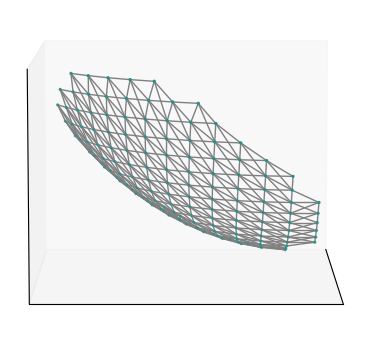
\includegraphics[width=0.95\textwidth]{empty-graph.png} 
        \caption{View on the graph nodes of an empty QUBIC patch with $nside = 16$. The map contains 141 nodes (green) and 492 edges (gray). }
        \label{fig:empty-graph}
    \end{minipage}\hfill
    \begin{minipage}{0.45\textwidth}
        \centering
        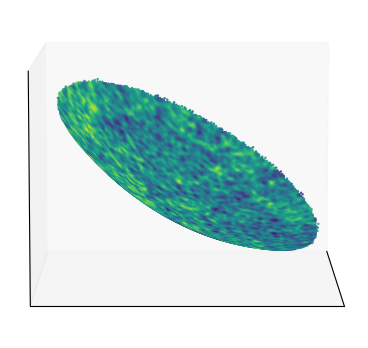
\includegraphics[width=0.95\textwidth]{graph-cmb.png} 
        \caption{View on the graph nodes of QUBIC patch with $nside = 256$. The map contains 34560 nodes and 136684 edges, each storing the sky amplitude and its relation to surrounding pixels. }
        \label{fig:graph-cmb}
    \end{minipage}
\end{figure}

The first type connects each pixel to its 8 neighbors on the sphere, as defined by the HEALPix pixel adjacency. Edge weights are Gaussian in the Euclidean distance between pixel centers \cite{gorski2005}. These edges carry spatial information and define the graph Laplacian used in the graph convolutions in Section~\ref{sec:architecture-loss}.

The second type connects pairs of pixels that appear in the same TOD sample, the ones that are mixed together in one projection. These are read from the sparse structure of the projection operator. For each TOD, the array stores the pixel indices of the nine sky pixels contributing to that mixing (the retained
synthesized beam peaks), and all unordered pixel pairs from each row are included as edges. It is important to note that these co-observed pixels are not geographic neighbors on the sky, they are separated by the distance between synthesized beam peaks. These edges carry the information needed for unmixing the projection.

All pixels are given in HEALPix NESTED ordering. The set of observed pixels is defined by the coverage map $c_p = L^T \cdot \mathbf{1}$, which is the number of TOD samples that contribute to each pixel weighted by beam amplitude. Coverage can be considered the number of times a pixel on the sky has been observed. We define the QUBIC patch as the set of pixels that have the coverage $c_p$ at least $2\%$ of its maximum value, and the pixels below this threshold are excluded from graphs. The number of nodes in the graph corresponds to the number of HEALPix pixels, depending on the $nside$ value. Example of an empty graph structure and one filled with signal are given on Fig.~\ref{fig:empty-graph} and \ref{fig:graph-cmb}.


\subsection{Analytical Inverses}
\label{subsec:exact-inverses}

The operators $U$, $T$, $A$, $F$, $I$, and $D$ are all diagonal or scalar operators, so their inverses are obtained by straightforward element-wise division.

The unit conversion operator $U$ converts the sky temperature in $\mu$K to
power per frequency W~m$^{-2}$~Hz$^{-1}$ with the Planck spectrum. For temperature fluctuations around the CMB temperature $T_{\rm CMB}$, the conversion factor is given with Eq.~\ref{eq:unit-conversion}. The inverse is then the division with the same factor $U^{-1} = 1/u(\nu)$.

The atmospheric transmission $T$ multiplies the signal by a scalar $t_{\rm atm}$. Currently this scalar is assumed to be constant. The inverse is the division $T^{-1} = 1/t_{\rm atm}$.

The aperture integration operator $A$ multiplies with the effective area $a$ of the horn array, and converts W~m$^{-2}$~Hz$^{-1}$ to W~Hz$^{-1}$
\begin{equation}
    a = N_h \pi r_{\rm eff}^2,
\end{equation}
where $N_h$ is the number of open horns and $r_{\rm eff}$ their effective radius. Its inverse is 
\begin{equation}
    A^{-1} = \frac{1}{N_h \pi r_{\rm eff}^2}
\end{equation}

The bandpass filter $F$ converts W~Hz$^{-1}$ to W by multiplying with the bandwidth $\Delta\nu$, and the bandwidth depends on the chosen number of sub-bands. Its inverse is
\begin{equation}
    F^{-1} = 1 / \Delta\nu.
\end{equation}

The instrumental transmission $I$ and flux density integration $D$ are diagonal operators for each of the detectors. The transmission $I$ is the product of all optical component transmissions and detector efficiencies, $\eta_d = \prod_k t_k \cdot \eta_{\rm det}$. The integration $D$ is the solid angle of each detector on the focal plane $d_{eff}$, depending on the structure of the secondary beams. Both are inverted element-wise, $I^{-1} = 1/\eta_d$ and $D^{-1} = 1/d_{\rm eff}$ per detector. The efficiency $\eta_d$ can be treated as a differentiable parameter and can be estimated from data during training, as it will be shown in Section~\ref{sec:probabilistic}.

\subsection{Half-Wave Plate and Polarizer}
\label{subsec:polarization}

After passing through the aperture and filters, the signal reaches the rotating half-wave plate and the polarizing grid. As seen in Section~\ref{subsec:acquisition}, these two operators act together, because the polarizer mixes the three Stokes parameters together depending on the angles of the HWP. Therefore, these operators are inverted together, since the information needed to undo this operation is written in the HWP modulation.

The HWP rotates by $-4\psi(t)$, as written in Eq.~\ref{eq:hwp}. This is applied to the $(I, Q, U)$ Stokes maps and gives
\begin{equation}
    \begin{pmatrix} I \\ Q' \\ U' \end{pmatrix}
    =
    \begin{pmatrix} 1 & 0 & 0 \\ 0 & \cos 4\psi & \sin 4\psi \\
    0 & -\sin 4\psi & \cos 4\psi \end{pmatrix}
    \begin{pmatrix} I \\ Q \\ U \end{pmatrix}.
\end{equation}

Afterwards, the polarizer combines these signals to a scalar by selecting the intensity and a polarization component by
\begin{equation}
    d = \tfrac{1}{2}\,I + \tfrac{1}{2}\bigl(\cos 4\psi\, Q + \sin 4\psi\, U\bigr),
    \label{eq:pol-scalar}
\end{equation}
The polarizer selection is written as $P_{\rm ol} = 0.5\begin{pmatrix}1 & 1 & 0\end{pmatrix}$ so the operation of the HWP and polarizer gives
\begin{equation}
    d(\psi) = P_{\rm ol}\,\mathrm{HWP}(\psi)
    \begin{pmatrix}I\\Q\\U\end{pmatrix}
    = \tfrac{1}{2}\Bigl(I + Q\cos4\psi + U\sin4\psi\Bigr).
    \label{eq:pol-single}
\end{equation}

A single TOD sample is only one linear combination of $(I,Q,U)$, so $P_{\rm ol}\,\mathrm{HWP}(\psi)$ is rank 1 and cannot be inverted. However, if the same sky pixel is observed at at least 3 different HWP angles $\psi_1,\dots,\psi_N$, we arrive at the system of linear equations
\begin{equation}
    \begin{pmatrix}d_1\\d_2\\ \vdots \\ d_N\end{pmatrix}
    = \tfrac{1}{2}
    \begin{pmatrix}
        1 & \cos4\psi_1 & \sin4\psi_1\\
        1 & \cos4\psi_2 & \sin4\psi_2\\
        \vdots & \vdots & \vdots\\
        1 & \cos4\psi_N & \sin4\psi_N
    \end{pmatrix}
    \begin{pmatrix}I\\Q\\U\end{pmatrix}
    \equiv P_H
    \begin{pmatrix}I\\Q\\U\end{pmatrix}.
    \label{eq:pol-stack}
\end{equation}
(here the combined operator is called $P_H$ for simplicity).
The matrix $P_H$ has the dimension of angles times 3. With 4 angles (distinct and evenly separated), $P_H^T P_H$ is full rank and invertible. The least-squares solution
\begin{equation}
    \begin{pmatrix}I\\Q\\U\end{pmatrix}
    = 2\,(P_H^T P_H)^{-1} P_H^T
    \begin{pmatrix}d_1\\d_2\\ \vdots \\ d_N\end{pmatrix}
\end{equation}
gives all three Stokes parameters at one pixel. Each additional HWP angle adds one more row to $P_H$, and the system becomes solvable with enough observations, which is also the function of HWP rotations in experiments that observe polarization maps.

\subsection{Detector Time Response}
\label{subsec:detector}

The TES bolometers convolve the signal with a truncated exponential, with a time constant $\tau$, as Eq.~\ref{eq:detector-response}. In this form, the operator is not invertible as the convolution destroys information. However, we know that in the Fourier domain this becomes a multiplication by
$B(\omega) = (1 + i\omega\tau)^{-1}$.  Here, the inverse is simply
\begin{equation}
    B^{-1}(\omega) = 1 + i\omega\tau.
    \label{eq:bolometer-inv}
\end{equation}
This deconvolution is implemented as a linear layer with a single parameter $\hat{\tau}$, which can be left fixed or learnable as a differentiable parameter. It is initialized to the instrument value and can be updated during training by backpropagation, as explained in Section~\ref{sec:probabilistic}. Because the layer architecture enforces the form Eq.~\ref{eq:bolometer-inv}, the network cannot learn nonphysical deconvolution kernels, and the fitted parameter corresponds exactly to the detector time constant.

\subsection{The Projection Operator}
\label{subsec:projection}

The projection $L$ maps the sky to TOD samples through the synthesized beam and is the most important process in an interferometric instrument. Each sample is a weighted sum of the sky values at the nine beam peaks,
\begin{equation}
    d_j = \sum_{k=1}^{9} w_{jk}\,s_{k},
    \label{eq:proj-sum}
\end{equation}
where $k$ are the pixels and $w_{jk}$ the peak amplitudes, for every TOD sample $j$. Because each TOD sample mixes the information coming from nine different sky pixels into one number, the projection is non-invertible (as it is usually with summation). 

Starting from Eq.~\ref{eq:forward}, the estimate for the sky from the maximum likelihood approach is
\begin{equation}
    s = (L^T L)^{-1} L^T d.
    \label{eq:maximumlikelihoodprojection}
\end{equation}
The matrix $L^T L$ has dimension $N_{\rm pix} \times N_{\rm pix}$ and
is too large to invert. We know from the acting of the projection operator that it is a mixing kernel. The inverse of a mixing is given with the Neumann series
\begin{equation}
    (I - \lambda K)^{-1} = \sum_{n=0}^{\infty} \lambda^n K^n.
    \label{eq:neumann}
\end{equation}
We can write the projection mixing as the sum of its diagonal and off-diagonal parts, $L^T L = D + O$. If we write this as  
\begin{equation}
    (D + O)^{-1}
    = (I + D^{-1}O)^{-1}D^{-1}
    \label{eq:projectiondoexpansion}
\end{equation}
we can then use the Neumann series to approximate the inverse of that mixing as
\begin{equation}
    (D + O)^{-1}
    = D^{-1} \sum_{k=0}^{\infty} (-D^{-1} O)^k
    = [ I - D^{-1}O + D^{-1}OD^{-1}O - \cdots ] D^{-1}
    \label{eq:neumanndo}
\end{equation}
which can be plugged back in to Eq.~\ref{eq:maximumlikelihoodprojection}. After exchanging the Neumann expression for the $(L^TL)^{-1}$, the estimate for the sky is
\begin{equation}
    s
    =\sum_{k=0}^{\infty} (-D^{-1} O)^k \cdot D^{-1} L^T d.
    \label{eq:maximumlikelihoodprojectionneumann}
\end{equation}
The term $D^{-1} L^T d$ is the back-projection normalized by coverage, which we call the dirty map $\tilde{s}_0$ or simply the back-projected map, and it is shown on Fig.~\ref{fig:backprojection}. Each higher-order term in Eq.~\ref{eq:neumann} gives additional information about the mixing, the terms at order $k$ give information $k$ connections away when looking at co-observed pixels, described in Section~\ref{subsec:graph}. When looking at the square mixing operator $L^TL = D + O$ , the higher order terms explain the values further away from the square diagonal. 

\begin{figure}[h]
\centering 
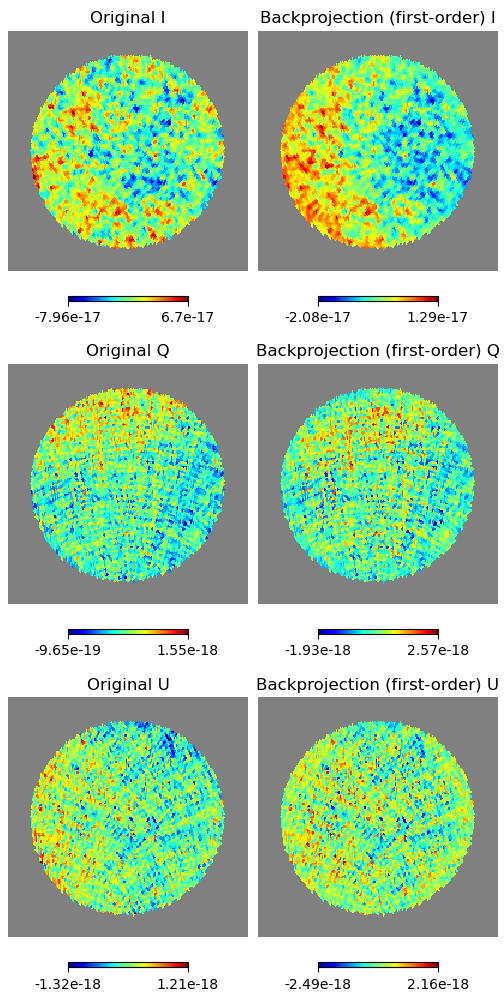
\includegraphics[width=.45\textwidth]{backprojection.png}
\caption{ Back-projection (or dirty sky) on an example simulated TOD. The first order correction recovers the center of the patch well, where diagonal terms of the projection operator are dominating. 
\label{fig:backprojection} }
\end{figure}

The Chebyshev graph filter of order $M$ is
\begin{equation}
    h(\tilde{L}) = \sum_{m=0}^{M} c_m T_m(\tilde{L}),
    \label{eq:cheb}
\end{equation}
where $T_m$ are Chebyshev polynomials of the graph Laplacian $\tilde{L}$ and $c_m$ are learnable coefficients. This corresponds exactly to Eq.~\ref{eq:neumann} and can be applied to the graph adjacency matrix \cite{defferrard2016chebconv}. The $M$ order of the adjacency matrix represents $M$ hops away from each node, or the number of connections one needs to pass before reaching a node of that order. In the algorithm, the order is limited to $M = 3$ because pixels separated by more than three connections between
synthesized beam peaks cannot contribute to the same TOD sample \cite{kardum2025proceeding}. Therefore, the higher order terms in Eq.~\ref{eq:cheb} are dropped, and the choice of the expansion order is given by geometry.

The full projection inverse is then
\begin{equation}
    L^{-1} \approx L^\dagger + R_\theta,
\end{equation}
where $L^\dagger = D^{-1}L^T$ is the fixed dirty map and $R_\theta$ is the trainable Chebyshev correction network, which will be explained in detail in Section~\ref{sec:architecture-loss}. The residual $R_\theta$ learns only the off-diagonal correction terms in Eq.~\ref{eq:neumann} that $L^\dagger$ does not depend on. Here, it is important to notice that only this correction factor up to the third order in an expansion series is learned, instead of a full TOD-to-sky inverse, which greatly simplifies the learning process and keeps all the architecture parameters and corrections interpretable, as explained in Section~\ref{subsec:residual-learning}.

\section{Network Architecture and Loss Functions}
\label{sec:architecture-loss}

One of the most important points in a physics-guided algorithm is the choice of architecture units inside the neural network. The layers have to be chosen so that their corresponding equations imitate the equations describing the acquisition procedure, or in this case its inverse. The neural network attempts to imitate the process given in Eq.~\ref{eq:inverse-separated}, with architectures of each separate module being chosen based on the physics behind the operator. 

As discussed in Section~\ref{subsec:implementation}, the analytical inverses from Section~\ref{subsec:exact-inverses} are implemented with PyTorch Linear Layers. Operators with no analytical inverse are explained below. 

\subsection{Architecture: \texttt{SharedCheb3Head}}
\label{subsec:net-arch}

As seen in Section~\ref{subsec:projection} and Fig.~\ref{fig:backprojection}, the back-projection $L^\dagger$ gives a starting estimate of the sky. The residual correction $R_\theta$ of Eq.~\ref{eq:residual} is computed with the higher order Neumann terms from Eq.~\ref{eq:neumann}. Therefore, we chose a graph neural
network (GNN) that operates on the observed sky patch 
\cite{scarselli2009gnn}.

The Neumann series $\sum_k (-D^{-1}O)^k$ is equivalent to a polynomial in the graph Laplacian
\cite{defferrard2016chebconv}, so the projection inverse is the Chebyshev polynomial from Eq.~\ref{eq:cheb}.

The network \texttt{SharedCheb3Head} processes all three Stokes maps together as a vector input $\tilde{s}_0 = (\tilde{I}, \tilde{Q}, \tilde{U}).$ The architecture has a shared encoder and three separate output heads
\begin{align}
    h_0 &= \text{ReLU}(\texttt{ChebConv}(3 \to 128,\, K=3)(x,\,
    \mathcal{E}_{\rm geo})), \\
    h_\ell &= \text{ReLU}(\texttt{ChebConv}(128 \to 128,\, K=3)
    (h_{\ell-1},\, \mathcal{E}_{\rm geo}) + h_{\ell-1}), \quad
    \ell = 1,2,3, \\
    \delta_X &= \texttt{ChebConv}(128 \to 1,\, K=3)(h_3,\,
    \mathcal{E}_{\rm geo}), \quad X \in \{I, Q, U\},
\end{align}
with a global residual connection giving the output
\begin{equation}
    \hat{s} = \tilde{s}_0 + [\delta_I,\, \delta_Q,\, \delta_U].
\end{equation}
The local skip connections $h_\ell = f(h_{\ell-1}) + h_{\ell-1}$ stabilize gradient flow. The shared encoder
processes I, Q, and U together so the polarization correlations coming from the HWP modulation are considered.  When the instrumental constants are fixed, the parameter count is less than 40 \cite{kardum2025proceeding}, compared with $\sim 11\times 10^6$ for a ResNet~\cite{he2016resnet} and $\sim 30\times 10^6$ for a U-Net~\cite{ronneberger2015unet} architecture.

\subsection{Loss Functions}
\label{subsec:losses}

Training the residual network requires comparing the predicted sky $\hat{s}$ to the true sky $s$ on supervised pairs from simulated data. Four loss terms are used, each from a different property of this reconstruction. 

\paragraph{Co-observed edge loss.}
The primary loss of the neural network is the Co-observed edge loss. The most physically motivated loss term makes sure the pairs of pixels that were simultaneously observed in the same TOD sample and mixed in one synthesized beam are consistent. The loss is defined as
\begin{equation}
    \mathcal{L}_{\rm coobs} = \frac{1}{|\mathcal{E}_{\rm coobs}|}
    \sum_{(i,j) \in \mathcal{E}_{\rm coobs}} \sum_X
    \left[(\hat{s}^X_i - \hat{s}^X_j) -
    (s^X_i - s^X_j)\right]^2.
    \label{eq:loss-coobs}
\end{equation}
Co-observed pixels are linked by the synthesized beam and are not spatially close. This loss supervises the unmixing of the projection. If two pixels are co-observed, their predicted difference must match their
true difference, as seen through the beam at each pointing, and 9 co-observed pixels cannot contribute to more than the input at that TOD sample when summed. 

\paragraph{Geometric edge loss.}
The synthesized beam introduces correlated residuals between nearby pixels on the sky due to its resolution not perfectly corresponding to the granularity of HEALPix maps. To regularize that, we penalize differences between the predicted and true differences across pixels and their closest neighbors in the HEALPix notation
\begin{equation}
    \mathcal{L}_{\rm geo} = \frac{1}{|\mathcal{E}_{\rm geo}|}
    \sum_{(i,j) \in \mathcal{E}_{\rm geo}} \sum_X
    \left[(\hat{s}^X_i - \hat{s}^X_j) -
    (s^X_i - s^X_j)\right]^2.
    \label{eq:loss-geo}
\end{equation}
This loss penalizes incorrect gradients across the map (rather than incorrect absolute values which is penalized with $\mathcal{L}_{\rm pix}$).


\paragraph{Pixel loss.}
The pixel-wise mean squared error on the scaled maps is defined as
\begin{equation}
    \mathcal{L}_{\rm pix} = \frac{1}{N_{\rm obs}}
    \sum_{p \in \mathcal{S}} \sum_{X \in \{I,Q,U\}}
    \left(\hat{s}^X_p - s^X_p\right)^2.
    \label{eq:loss-pix}
\end{equation}
and is a standard supervised reconstruction loss. It makes sure the network gives correct values per pixel in average. Due to its tendency to not penalize correct average values, pixel losses alone tend to smooth the maps. This is correctly handled by previously described losses $\mathcal{L}_{\rm geo}$ and $\mathcal{L}_{\rm coobs}$.


\paragraph{Physics loss.}
The fourth loss term reapplies the forward projection operator to the predicted sky and compares it with the
observed TOD. The back-projected TOD and simulated skies are compared as
\begin{equation}
    \mathcal{L}_{\rm phys} = \frac{1}{N_{\rm TOD}}
    \left\| L\bigl(\hat{s}_{\rm phys}\bigr) - d_{\rm obs}
    \right\|^2,
    \label{eq:loss-phys}
\end{equation}
where $d_{\rm obs}$ is the scalar TOD. Comparison of the simulated TOD and its corresponding sky closely imitates the forward modeling approaches described in Section~\ref{sec:forward}, and the penalization in this loss is closely related to PCG methods from Section~\ref{subsec:pcg-method}. This ensures the estimated sky can definitely produce the instrument response measured in QUBIC, and is added together with $\mathcal{L}_{\rm pix}$ for completeness and interpretability. 

\paragraph{Combined loss and weighting.}
The total loss is
\begin{equation}
    \mathcal{L} = \lambda_{\rm pix}\,\mathcal{L}_{\rm pix}
    + \lambda_{\rm geo}\,\mathcal{L}_{\rm geo}
    + \lambda_{\rm coobs}\,\mathcal{L}_{\rm coobs} +  \lambda_{\rm phys}\,\mathcal{L}_{\rm phys},
    \label{eq:loss-total}
\end{equation}
with $\lambda$ being weighting factors for each loss. Since the Q and U maps have amplitudes
around $10^3$ times smaller than I, an additional weight $w_{QU} = 10^3$ is applied to the Q and U contributions in $\mathcal{L}_{\rm geo}$ and $\mathcal{L}_{\rm coobs}$ as an initialization.

\subsection{Training Strategy}
\label{subsec:training}

Training data consist of pairs of back-projected dirty skies and true skies, generated by running the
QUBICsoft simulation for different sky realizations. All analytical inverses are applied prior to resolving residuals, to produce realistic intermediate maps or TODS. The QUBICsoft gives the exact forward model and is used to create TODs as well as all intermediate quantities in the chain Eq.~\ref{eq:forward} for evaluating $\mathcal{L}_{\rm phys}$.

The network is optimized with Adam and a step learning rate schedule. Training is done in rotating stages with rotating loss weights. 

The gradients of the learning are inspected at each step. The gradients are constant in fixed analytical inverses, and diminishing in inverses with residual learning. The convergence of the gradient is used to adjust the parameters of the Adam optimizer. 

\section{Monochromatic Reconstruction}
\label{sec:validation-mono}

We now reproduce the setup and results from \cite{kardum2025proceeding}, by validation with a monochromatic pipeline from Sections~\ref{sec:modular} and~\ref{sec:operators}.

\subsection{Reconstruction Accuracy and Conditioning Improvement}
\label{subsec:accuracy}

We evaluated the algorithm on simulated data. We create QUBIC TODs at $150$~GHz from generated $I,Q,$ and $U$ skies with the QUBICsoft forward model described in Section~\ref{subsec:acquisition}. The training is described in Section~\ref{subsec:training}. We compare noiseless reconstruction of skies generated with the same seed, so that there is no difference coming from different random realizations, and with the same coverage. Fig.~\ref{fig:mono-reconstruction} shows the simulated input sky, the reconstruction, and the resulting error for PCG and this work. 

\begin{figure}[h]
\centering
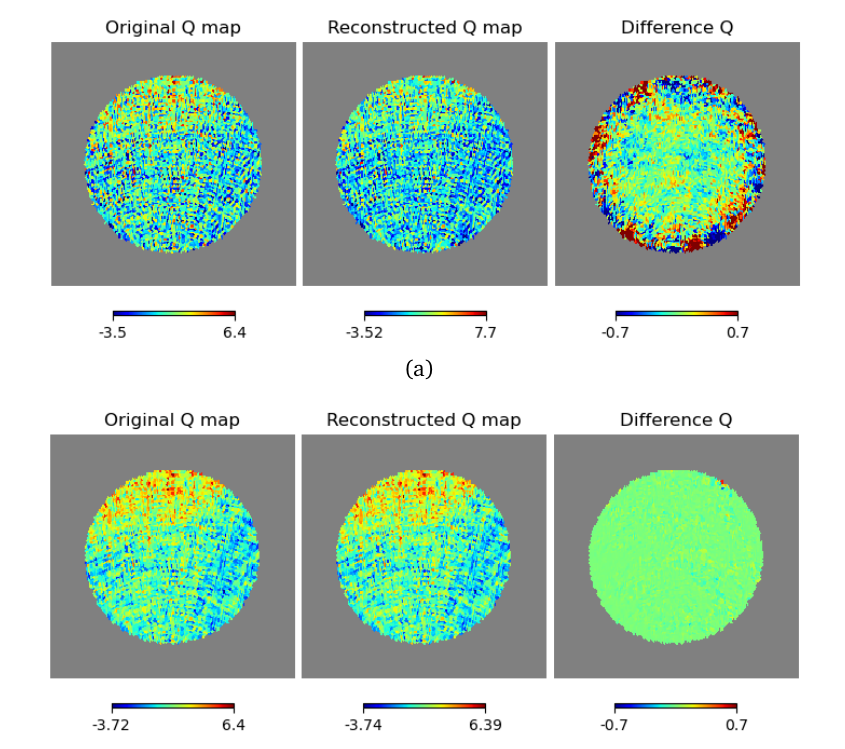
\includegraphics[width=.75\textwidth]{reconstruction-comparison.png}
\caption{\label{fig:mono-reconstruction} Simulated sky (Q polarization), the reconstructed sky, and the reconstruction error, for the PCG method (Section~\ref{subsec:pcg-method}) and the proposed modular network (Section~\ref{subsec:net-arch}). Taken from \cite{kardum2025proceeding}.}
\end{figure}

The reconstruction error of the modular network is lower than that of PCG across all skies, with the largest improvement near the edge of the observed patch. Because $R_\theta$ operates directly on the co-observed-pixel graph of Section~\ref{subsec:graph} instead of on pixels cumulatively, it propagates information of the true mixing structure of the synthesized beam even in low coverage regions with an explicit correction, which PCG recovers only implicitly.

\subsection{Comparison to PCG}
\label{subsec:comparison-pcg}

Apart from improvement of reconstruction error seen on Fig.~\ref{fig:mono-reconstruction}, the comparison with forward methods has additional advantages of iteration cost, reusability, and interpretability.

Forward models require repeated forward and transpose calculations of the full operator $H$ per reconstructed sky, with the number of iterations to convergence increasing with the condition number of $H^TN^{-1}H$. Because the modular network runs a single forward pass through Eq.~\ref{eq:inverse-separated}, with the only ill-conditioned step handled by the fixed correction terms, reconstruction cost does not scale with the condition number.

As mentioned in Section~\ref{subsec:pcg-method}, a PCG solution is specific to one realization of $d$ and must be rerun in full for any change in noise realization, sky, or instrumental parameters. The modular network, once trained, is a fixed function of $d$ that can be applied directly to new TODs without retraining, and, as discussed in Section~\ref{subsec:implementation}, individual modules (such as the example $\eta$ from Section~\ref{sec:probabilistic}) can be updated independently without retraining the correction terms.

Finally, every module of Eq.~\ref{eq:inverse-separated} corresponds to a physical operation, so intermediate outputs (e.g.\ the deconvolved-only TOD, or the dirty map $\tilde s_0$ before the residual correction) are physically meaningful and can be inspected. This is what makes possible to additionally recover instrumental parameters with uncertainty, in the same pipeline, as presented in Section~\ref{sec:probabilistic}. In comparison, this is not possible with forward models which return only the final maximum-likelihood sky with no intermediate physical quantities.


\section{Probabilistic Instrument Parameters}
\label{sec:probabilistic}

Several of the analytical and physics-guided inverses described in Section~\ref{sec:operators} depend on instrumental constants that are only known up to some calibration uncertainty: the detector efficiency $\eta_d$ in the transmission operator $I^{-1}$ (Section~\ref{subsec:exact-inverses}) and the bolometer time constant $\hat{\tau}$ in $B^{-1}$ (Section~\ref{subsec:detector}) are the two treated in this work, though the same treatment applies to any other scalar parameter entering the chain. So far, these have been used as fixed or point-estimated differentiable parameters, updated by backpropagation together with the residual network $R_\theta$. Because every module in the inverse chain of Eq.~\ref{eq:inverse-separated} is implemented as a differentiable PyTorch layer, the same computational graph can be reused to find the full distribution of values consistent with the data. This is then used to find the uncertainty and investigate how it propagates into the reconstructed maps.

\subsection{Variational Inference with Pyro}
\label{subsec:pyro}

We use Pyro \cite{bingham2019pyro}, a probabilistic programming library built on PyTorch, to transform an instrumental parameter $\theta$ (such as $\eta_d$ or $\tau$) from a fixed value to a random variable. With a predefined prior $p(\theta)$, we infer its posterior $p(\theta \mid d)$ from an observed or simulated TOD. Because Pyro tensors are ordinary PyTorch tensors, the analytical-inverse layers from Section~\ref{subsec:exact-inverses} don't need special treatment. The modules are wrapped in a PyroModule, and the constant are replaced by a PyroSample drawn from $p(\theta)$. Therefore, the forward pass through the layer doesn't change except that $\theta$ is now sampled and not fixed.

The posterior $p(\theta \mid d)$ is approximated with Stochastic Variational Inference (SVI). From SVI, AutoNormal creates a Gaussian (for assumed normal distributions) which is optimized to match the true posterior by maximizing the Evidence Lower Bound (ELBO). The maximization is again done with the Adam optimizer. This training loop has the same structure as the one described in Section~\ref{subsec:training} for $R_\theta$, and can be run together with it, enabling the residuals and the instrumental parameters to be adjusted at the same time from the same data. Once trained, posterior samples of parameters are drawn from the guide with Pyro's Predictive utility. The drawing returns the best estimate as well as the spread of the distribution which corresponds to the uncertainty of that instrumental parameter. This can be retrieved for any uncertain instrumental parameter and can be propagated downwards in the Sequential network.

The forward methods given in Section~\ref{sec:forward} also provide an uncertainty on the reconstructed map, often referred to as noise. However, these methods return a single uncertainty per pixel with no underlying explanation to the source of its spread. Propagating the uncertainty from Pyro through distinct modules from Eq.~\ref{eq:inverse-separated} allows us to quantify the influence on the uncertainty from separate algorithm parts, and therefore connect them to different physical processes in the acquisition. Investigation of posterior distributions on instrumental parameters also gives direct insight into the correctness of our assumptions regarding their values. A narrow posterior shows the data supports the assumed value of the parameter $\theta$.

\subsection{Recovering the Detector Efficiency}
\label{subsec:pyro-results}

As an example, we will change the detector efficiency $\eta_d$, described in Section~\ref{subsec:exact-inverses}, to a variable and recover its posterior from pairs of simulated TODs before and after applying the operator $I$. We use a Pyro.plate over the batch of samples. For this example, ten TODs are simulated, half with $\eta_d^{(1)} = 0.8$ and half with $\eta_d^{(2)} = 0.7$. After initializing the AutoNormal guide and the Adam optimizer, the ELBO is minimized on 400 SVI steps. The samples are returned from Pyro.Predictive and correspond well to simulated values in the set of simulated TODs, as seen on Fig.~\ref{fig:efficiency-mean}.

\begin{figure}[h]
    \centering
    \begin{minipage}{0.45\textwidth}
        \centering
        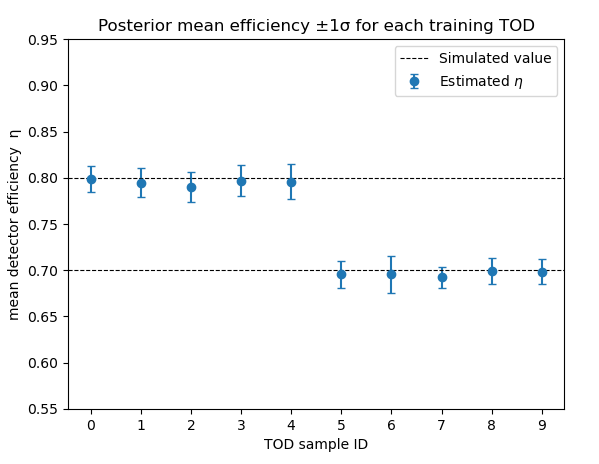
\includegraphics[width=0.95\textwidth]{efficiency-mean.png} 
        \caption{The mean posterior efficiencies per sample, inferred with Pyro and compared to their true values.}
        \label{fig:efficiency-mean}
    \end{minipage}\hfill
    \begin{minipage}{0.45\textwidth}
        \centering
        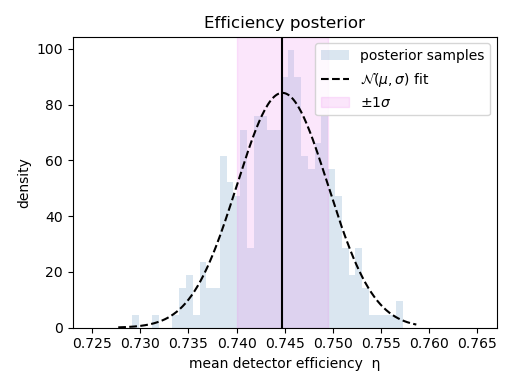
\includegraphics[width=0.95\textwidth]{efficiency-posterior.png} 
        \caption{Posterior distribution from drawn samples of efficiency, on a simulated set of TODs, drawn with Pyro.Predictive.}
        \label{fig:efficiency-posterior}
    \end{minipage}
\end{figure}

We inspect the posterior by drawing a large number of samples. For an assumed unique value for $\eta_d$ and assumed normal distribution, we recover a posterior seen in Fig.~\ref{fig:efficiency-posterior}, showing the recovered posterior mean and $1\sigma$ band for each training sample. This confirms that the differentiable implementation of $I^{-1}$ is precise and can be used for gradient-based inference to recover the parameter it depends on, as well as a meaningful uncertainty, from the same forward chain used for map reconstruction. This requires no substantial change to the reconstruction network. The same procedure applies unchanged to $\tau$ in $B^{-1}$, and to any calibration constant entering an analytical or physics-guided inverse in Eq.~\ref{eq:inverse-separated}.

\section{Conclusion}
\label{sec:conclusion}

We have presented a physics-guided neural architecture for QUBIC map-making that inverts the acquisition operator of Eq.~\ref{eq:operator-chain} module by module.

On monochromatic reconstruction, this reduces the condition number and lowers the reconstruction error (compared to PCG) on all three Stokes parameters. This approach also requires orders of magnitude fewer parameters than comparable data-driven architectures. The same architecture is applicable to multi-band spectral imaging, where the coupling between sub-bands from the frequency-dependent synthesized beam is handled with the same modular structure. Because the pipeline is fully differentiable and physically interpretable in every module, it enables variable instrumental parameters. Systematic constants that are usually fixed at some values can instead be treated as variables and inferred with  uncertainty, by using variational inference (Section~\ref{sec:probabilistic}).

The central idea of factorizing a known measurement process into its physical components and reserving learning capacity only for the operators that are ill-conditioned, is not specific to bolometric interferometry. The algorithm can be readjusted to any physical experiment.  We can conclude that this is a mixture between fully analytical map-making and fully data-driven neural network reconstruction. We keep the interpretability and reusability of the analytical approach while using the great computational efficiency and elegance of neural networks.

\begin{thebibliography}{99}

\bibitem{hamilton2022qubic1}
J.-C. Hamilton et al.,
\emph{QUBIC~I: Overview and science program},
\emph{JCAP} {\bf 04} (2022) 034,
[\href{https://arxiv.org/abs/2011.02213}{arXiv:2011.02213}].

\bibitem{mousset2022qubic2}
L. Mousset et al.,
\emph{QUBIC~II: Spectral polarimetry with bolometric interferometry},
\emph{JCAP} {\bf 04} (2022) 035,
[\href{https://arxiv.org/abs/2010.15119}{arXiv:2010.15119}].

\bibitem{torchinsky2022qubic3}
S.A. Torchinsky et al.,
\emph{QUBIC~III: Laboratory characterization},
\emph{JCAP} {\bf 04} (2022) 036,
[\href{https://arxiv.org/abs/2101.06036}{arXiv:2101.06036}].

\bibitem{regnier2024freqmaps}
M. Regnier et al.,
\emph{Spectral imaging with QUBIC: building frequency maps from
time-ordered-data using bolometric interferometry},
\emph{JCAP} {\bf 05} (2026) 032,
[\href{https://arxiv.org/abs/2409.18698}{arXiv:2409.18698}].

\bibitem{regnier2024spectral}
M. Regnier et al.,
\emph{Spectral imaging with QUBIC: building astrophysical components from
time-ordered-data using bolometric interferometry},
\href{https://arxiv.org/abs/2409.18714}{arXiv:2409.18714}.

\bibitem{kaasschieter1988}
E.F. Kaasschieter,
\emph{Preconditioned conjugate gradients for solving singular systems},
\emph{J. Comput. Appl. Math.} {\bf 24} (1988) 265.

\bibitem{kardum2025proceeding}
L. Kardum,
\emph{Architecturally constrained solutions to ill-conditioned problems
in QUBIC},
\emph{SciPost Phys. Proc.} (2025),
[\href{https://arxiv.org/abs/2510.00090}{arXiv:2510.00090}].

\bibitem{mousset2021thesis}
L. Mousset,
\emph{Exploring the primordial universe, inflation and primordial
gravitational waves with QUBIC, the Q\,\&\,U Bolometric Interferometer
for Cosmology},
Ph.D. thesis, Universit\'{e} Paris Cit\'{e} (2021),
\url{http://www.theses.fr/2021UNIP7133}.

\bibitem{gorski2005}
K.M. G\'{o}rski, E. Hivon, A.J. Banday, B.D. Wandelt, F.K. Hansen, M. Reinecke and M. Bartelmann,
\emph{HEALPix: A framework for high-resolution discretization and fast analysis of data distributed on the sphere},
\emph{Astrophys. J.} {\bf 622} (2005) 759,
[\href{https://arxiv.org/abs/astro-ph/0409513}{arXiv:astro-ph/0409513}].

\bibitem{scarselli2009gnn}
F. Scarselli, M. Gori, A.C. Tsoi, M. Hagenbuchner and G. Monfardini,
\emph{The graph neural network model},
\emph{IEEE Trans. Neural Netw.} {\bf 20} (2009) 61.

\bibitem{defferrard2016chebconv}
M. Defferrard, X. Bresson and P. Vandergheynst,
\emph{Convolutional neural networks on graphs with fast localized spectral filtering},
in \emph{Proceedings of the 30th International Conference on Neural Information Processing Systems}, NIPS'16, Curran Associates Inc. (2016), pp.~3844--3852.

\bibitem{he2016resnet}
K. He, X. Zhang, S. Ren and J. Sun,
\emph{Deep residual learning for image recognition},
in \emph{2016 IEEE Conference on Computer Vision and Pattern Recognition (CVPR)} (2016), pp.~770--778.

\bibitem{ronneberger2015unet}
O. Ronneberger, P. Fischer and T. Brox,
\emph{U-Net: Convolutional networks for biomedical image segmentation},
in \emph{Medical Image Computing and Computer-Assisted Intervention -- MICCAI 2015}, N. Navab, J. Hornegger, W.M. Wells and A.F. Frangi eds., Springer International Publishing (2015), pp.~234--241.

\bibitem{bingham2019pyro}
E. Bingham, J.P. Chen, M. Jankowiak, F. Obermeyer, N. Pradhan, T. Karaletsos, R. Singh, P. Szerlip, P. Horsfall and N.D. Goodman,
\emph{Pyro: Deep universal probabilistic programming},
\emph{J. Mach. Learn. Res.} {\bf 20} (2019) 1,
[\href{https://arxiv.org/abs/1810.09538}{arXiv:1810.09538}].

\end{thebibliography}


% Please avoid comments such as "For a review'', "For some examples",
% "and references therein" or move them in the text. In general,
% please leave only references in the bibliography and move all
% accessory text in footnotes.

% Also, please have only one work for each \bibitem.


\end{document}
